\documentclass[a5paper,ngerman]{scrartcl}
\usepackage{fontspec}
\setmainfont[Mapping=tex-text]{Vollkorn}
\setsansfont[Mapping=tex-text]{Vollkorn}
\setmonofont{Vollkorn}
\PassOptionsToPackage{normalem}{ulem}
\usepackage{ulem}
\usepackage{tikz}
\usetikzlibrary{positioning,fadings,through}
\usetikzlibrary{patterns}
\definecolor{balken}{HTML}{bbbbbb}
\definecolor{balken_border}{HTML}{888888}

\usepackage{enumitem,amssymb}
\usepackage{wasysym}
\usepackage{xcolor}
\usepackage{eso-pic}
\pagestyle{empty}
\usepackage[left=1cm,right=1cm,top=0.5cm,bottom=0.5cm,includeheadfoot]{geometry}
\renewcommand*{\sectionformat}{}

\AddToShipoutPicture*{% nur auf der aktuellen/nächsten Seite 
  \AtPageCenter{% In der Mitte der Seite 
    \put(\LenToUnit{-.5\paperwidth},0){% eine halbe Seite links und damit jetzt am linken Rand 
       \line(1,0){\LenToUnit{0.1cm}}% 2cm lange Linie 
    }%
  }%
}
% defining the new dimensions and parameters
\newlength{\hatchspread}
\newlength{\hatchthickness}
\newlength{\hatchshift}
\newcommand{\hatchcolor}{}
% declaring the keys in tikz
\tikzset{hatchspread/.code={\setlength{\hatchspread}{#1}},
hatchthickness/.code={\setlength{\hatchthickness}{#1}},
hatchshift/.code={\setlength{\hatchshift}{#1}},% must be >= 0
hatchcolor/.code={\renewcommand{\hatchcolor}{#1}}}
% setting the default values
\tikzset{hatchspread=3pt,
hatchthickness=0.4pt,
hatchshift=0pt,% must be >= 0
hatchcolor=balken}

\pgfdeclarepatternformonly[\hatchspread,\hatchthickness,\hatchshift,\hatchcolor]% variables
{custom north east lines}% name
{\pgfqpoint{\dimexpr-2\hatchthickness}{\dimexpr-2\hatchthickness}}% lower left corner
{\pgfqpoint{\dimexpr\hatchspread+2\hatchthickness}{\dimexpr\hatchspread+2\hatchthickness}}% upper right corner
{\pgfqpoint{\dimexpr\hatchspread}{\dimexpr\hatchspread}}% tile size
{% shape description
\pgfsetlinewidth{\hatchthickness}
\pgfpathmoveto{\pgfqpoint{\dimexpr\hatchshift-0.15pt}{-0.15pt}}
\pgfpathlineto{\pgfqpoint{\dimexpr\hatchspread+0.15pt}{\dimexpr\hatchspread-\hatchshift+0.15pt}}
\ifdim \hatchshift > 0pt
\pgfpathmoveto{\pgfqpoint{-0.15pt}{\dimexpr\hatchspread-\hatchshift-0.15pt}}
\pgfpathlineto{\pgfqpoint{\dimexpr\hatchshift+0.15pt}{\dimexpr\hatchspread+0.15pt}}
\fi
\pgfsetstrokecolor{\hatchcolor}
%    \pgfsetdash{{1pt}{1pt}}{0pt}% dashing cannot work correctly in all situation this way
\pgfusepath{stroke}
}

\definecolor{bier_0}{HTML}{FDFE48}
\definecolor{bier_1}{HTML}{FEB437}
\definecolor{bier_2}{HTML}{F8842F}
\definecolor{bier_3}{HTML}{CE5924}
\definecolor{bier_4}{HTML}{BC5922}
\definecolor{bier_5}{HTML}{9B411C}
\definecolor{bier_6}{HTML}{742912}
\definecolor{bier_7}{HTML}{6C2511}
\definecolor{bier_8}{HTML}{381209}
\definecolor{bier_9}{HTML}{240004}

\newcommand{\Note}{\hfill$\square\,1$ $\square\,2$ $\square\,3$ $\square\,4$ $\square\,5$ $\square\,6$}
\newcommand{\Crit}[1]{\emph{#1:}~}
\newcommand{\Balken}{%
  \hspace{0.04\textwidth}
  \begin{tikzpicture}
	\setlength{\hatchthickness}{0.1pt}
    \fill[pattern=custom north east lines] (0.00\textwidth,0) rectangle (0.7\textwidth, 0.20);
	\setlength{\hatchthickness}{0.15pt}
    \fill[pattern=custom north east lines] (0.05\textwidth,0) rectangle (0.7\textwidth, 0.20);
	\setlength{\hatchthickness}{0.2pt}
    \fill[pattern=custom north east lines] (0.1\textwidth,0) rectangle (0.7\textwidth, 0.20);
	\setlength{\hatchthickness}{0.4pt}
    \fill[pattern=custom north east lines] (0.3\textwidth,0) rectangle (0.7\textwidth, 0.20);
	\setlength{\hatchthickness}{0.6pt}
    \fill[pattern=custom north east lines] (0.4\textwidth,0) rectangle (0.7\textwidth, 0.20);
	\setlength{\hatchthickness}{0.8pt}
    \fill[pattern=custom north east lines] (0.5\textwidth,0) rectangle (0.7\textwidth, 0.20);
	\setlength{\hatchthickness}{1.0pt}
    \fill[pattern=custom north east lines] (0.6\textwidth,0) rectangle (0.7\textwidth, 0.20);
	\setlength{\hatchthickness}{1.20pt}
    \fill[pattern=custom north east lines] (0.7\textwidth,0) rectangle (0.7\textwidth, 0.20);
    \draw[color=black, line width=0.05mm] (0,0) rectangle (0.7\textwidth, 0.2);
  \end{tikzpicture}
}

\makeatletter
\renewcommand*\section{\@startsection{section}{1}{\z@}%
{-0.5ex \@plus -1ex \@minus -.2ex}%
{0.5ex \@plus.2ex}%
{\raggedsection\large\bfseries\scshape\nobreak}%
}
\renewcommand*\subsection{\@startsection{subsection}{2}{\z@}%
{-0.25ex\@plus -1ex \@minus -.2ex}%
{0.25ex \@plus .2ex}%
{\raggedsection\normalsize\bfseries\scshape\nobreak}%
}
\makeatother

\usepackage{xunicode}
\usepackage{polyglossia}
\setdefaultlanguage[variant=german,spelling=new,babelshorthands=true]{german}

\begin{document}
{%
\Huge
\begin{center}
\textbf{Bierbewertungsbogen}
\end{center}
}%

\begin{minipage}[t]{0.47\textwidth}
\section{Grundsächliches}
\Crit{Dein Name}\uline{\hfill}
\Crit{Brauerei}\uline{\hfill} \\
\Crit{Biername}\uline{\hfill}
\Crit{Sorte}\uline{\hfill}\\
\Crit{Aktuelle Trunkenheit\textsuperscript{\tiny 1}}\uline{\hfill}\permil \\
\Crit{Wirtshaus}\uline{\hfill} \\
{\tiny \textsuperscript{1} sei ehrlich.}
\end{minipage}
\hfill\begin{minipage}[t]{0.47\textwidth}
\section{Das Äußere}
\Crit{Farbe}\hfill
\tikz\draw[black,fill=bier_0] (0,0) circle (.8ex);
\tikz\draw[black,fill=bier_1] (0,0) circle (.8ex);
\tikz\draw[black,fill=bier_2] (0,0) circle (.8ex);
\tikz\draw[black,fill=bier_3] (0,0) circle (.8ex);
\tikz\draw[black,fill=bier_4] (0,0) circle (.8ex);
\tikz\draw[black,fill=bier_5] (0,0) circle (.8ex);
\tikz\draw[black,fill=bier_6] (0,0) circle (.8ex);
\tikz\draw[black,fill=bier_7] (0,0) circle (.8ex);
\tikz\draw[black,fill=bier_8] (0,0) circle (.8ex);
\tikz\draw[black,fill=bier_9] (0,0) circle (.8ex);
\\
\Crit{Klarheit}\hfill $\square$ klar $\square$ nebelig $\square$ trüb\\
\Crit{Schaumkrone\textsuperscript{\tiny 2}}\uline{\hfill} \\
\Crit{Note}\Note \\
{\tiny \textsuperscript{2} (zB: feinporig, grobporig, kaum, lange anhaltend)}
\end{minipage}
\vspace{0.5cm}

\begin{minipage}[t]{0.47\textwidth}
\section{Geruch}
\Crit{Intensität}\Balken \\
\Crit{Balance}\hspace{0.26cm}\Balken \\  % süß / bitter.
\Crit{Malzaroma\textsuperscript{\tiny 3}}\uline{\hfill} \\
\Crit{Hopfenaroma\textsuperscript{\tiny 4}}\uline{\hfill} \\
\Crit{Note}\Note \\
{%
\textsuperscript{\tiny 3}\tiny (zB: Getreide, Brot, Süß, Toast, Nuss, Karamell, Schoko, Kaffee)
}%
\end{minipage}
\hfill\begin{minipage}[t]{0.47\textwidth}
\section{Mundgefühl}
\Crit{Viskosität}\hfill$\square$ leicht $\square$ mittel $\square$ ölig \\
\Crit{Kohlensäure\textsuperscript{\tiny 5}}\uline{\hfill} \\
\Crit{Empfindung\textsuperscript{\tiny 6}}\uline{\hfill} \\
\Crit{Note}\Note \\
{%
\vfill
\textsuperscript{\tiny 4}\tiny (zB: erdig, blumig, würzig, harzig, zitrus, fruchtig, chemisch)
}%
\end{minipage}

\vspace{0.6cm}
\begin{minipage}[t]{0.47\textwidth}
\section{Antrunk}
\Crit{Intensität}\Balken \\
\Crit{Balance}\hspace{0.26cm}\Balken \\  % süß / bitter.
\Crit{Malzgeschmack\textsuperscript{\tiny 3}}\uline{\hfill} \\
\Crit{Hopfengeschmack\textsuperscript{\tiny 4}}\uline{\hfill} \\
\Crit{Note}\Note \\
\vspace{0.1cm}
{%
\textsuperscript{\tiny 5}\tiny (zB: schal, spritzig, stark, feinperlend)
}%
\end{minipage}
\hfill\begin{minipage}[t]{0.47\textwidth}
\section{Nachtrunk}
\Crit{Intensität}\Balken \\
\Crit{Balance}\hspace{0.26cm}\Balken \\  % süß / bitter.
\Crit{Malzgeschmack\textsuperscript{\tiny 3}}\uline{\hfill} \\
\Crit{Hopfengeschmack\textsuperscript{\tiny 4}}\uline{\hfill} \\
\Crit{Note}\Note \\
\vspace{0.1cm}
{%
\textsuperscript{\tiny 6}\tiny (zB: cremig, warm, kreidig, süffig, sauer, prickelnd, erwärmend)
}%
\end{minipage}


\vfill
\vspace{0.6cm}
\begin{minipage}[t][4cm]{0.45\textwidth}
\section{Gesamt}
\Crit{Persönlicher Geschmack}~\hfill$\square$ Ja $\square$ Nein \\
\Crit{Katerverdächtig}~\hfill$\square$ Ja $\square$ Nein \\
\Crit{Bedienung} {\small $\square$ originell $\square$ nett \\ $\square$ rothaarig $\square$ aufmerksam \\ $\square$ hat alles?} \\
\vfill
\textbf{Gesamtnote:}\uline{\hfill}
\end{minipage}
\begin{minipage}[t]{0.5\textwidth}
\vfill
\hfill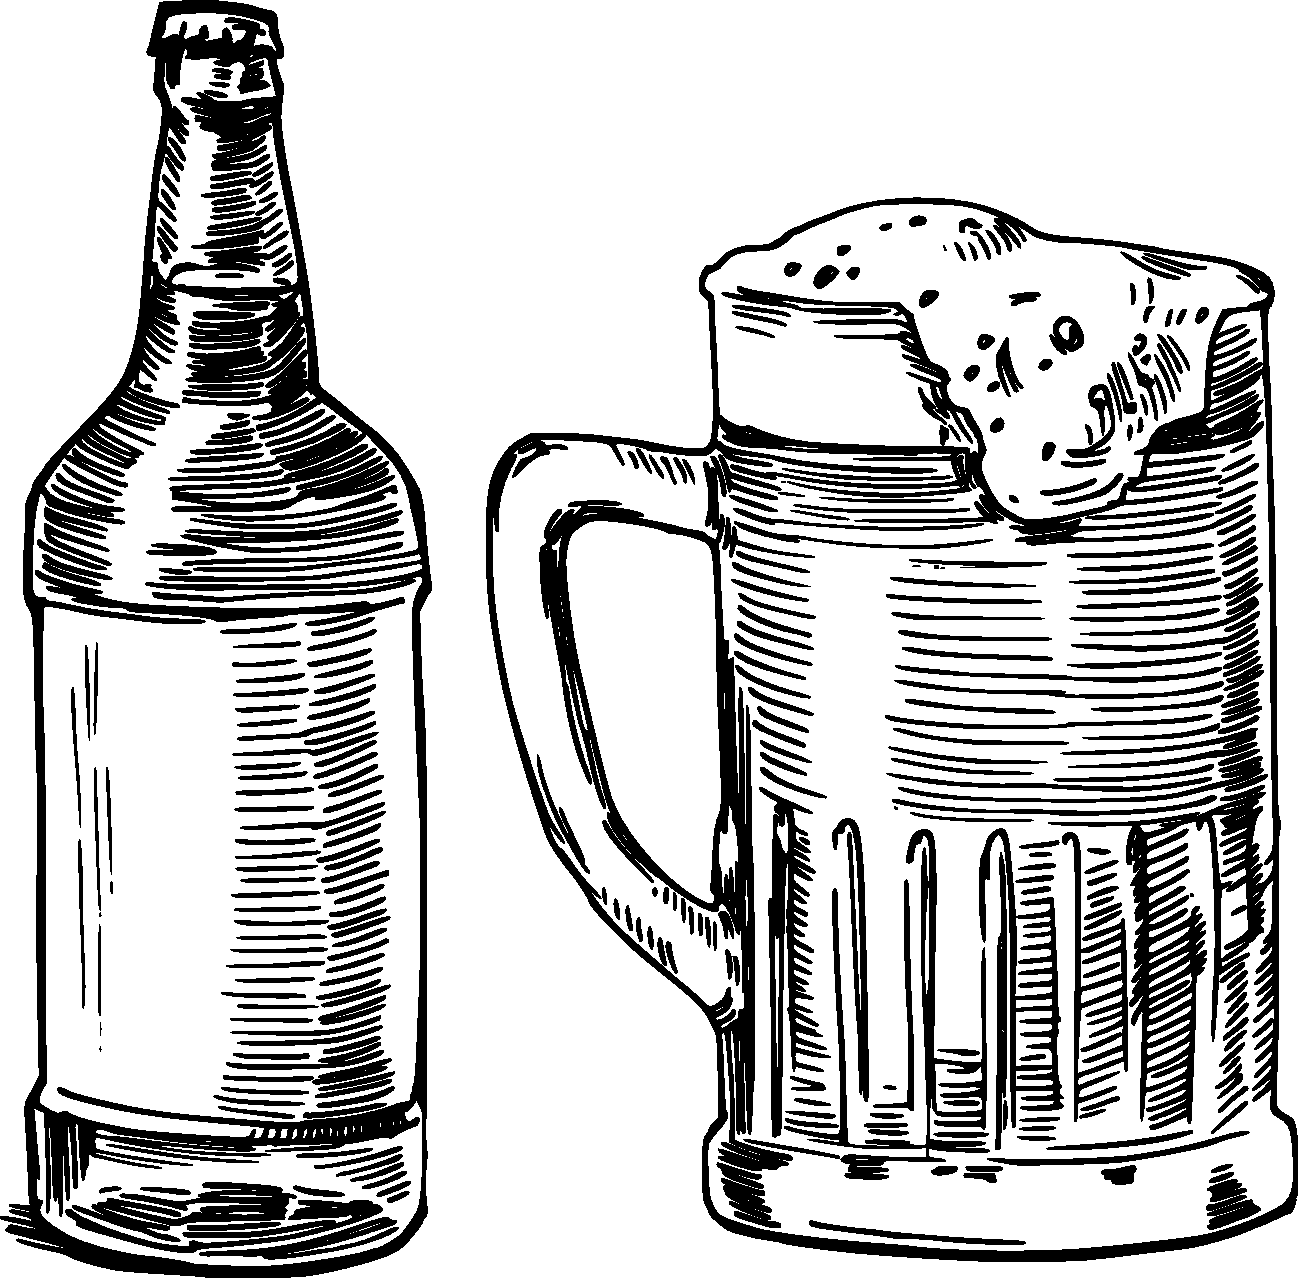
\includegraphics[width=0.7\textwidth]{bier-zeichnung.pdf}
\end{minipage}

\end{document}
